% !TEX encoding = UTF-8 Unicode
% !TEX root = rapport.tex

\chapter{Les conséquences d'évolutions divergentes}
Du constat de la dichotomie dans l'intégration de la technologie par la société et par l'éducation, émerge un questionnement : quelles sont les conséquences de ce décalage pour les individus ?


\section{Taux de chômage des jeunes}
Commençons tout d'abord par examiner les données du chômage des jeunes comparées aux données globales du chômage.
\begin{figure}[H]
\centering
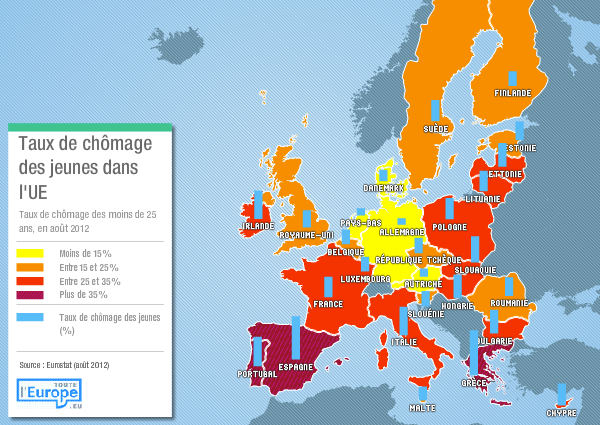
\includegraphics[width=0.92\linewidth]{figures/chom_jeunes}
\caption{Taux de chômage des jeunes dans l'UE en août 2012 \cite{chom_jeunes}}
\end{figure}

\begin{figure}[H]
\centering
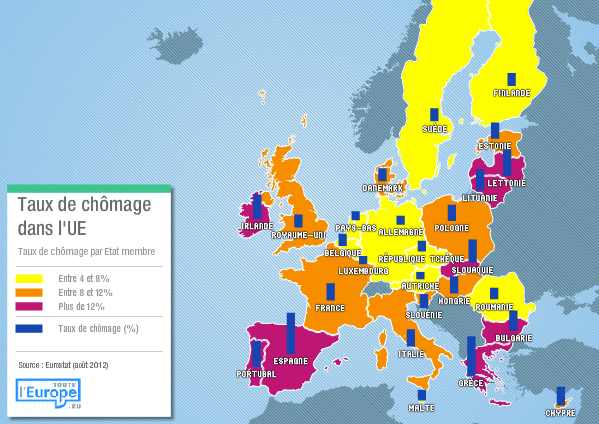
\includegraphics[width=0.92\linewidth]{figures/chom}
\caption{Taux de chômage dans l'UE en août 2012 \cite{chom}}
\end{figure}

\subsection{La formation des étudiants en inadéquation avec les besoins de la société / de l'industrie}
Le taux de chômage des jeunes a de nombreuses explications dont certaines économiques. Nous pensons néanmoins que les causes dues à une formation inadaptée ne sont pas négligeables.



\section{Les retombées imprévues de l'utilisation des technologies de la communication}

\subsection{Piège de Facebook pour les jeunes}



\section{Décrochages et échecs scolaires}
\subsection{La formation des étudiants en inadéquation avec leurs attentes}


\subsection{Hyperactivité chez les gamins qui ont juste besoin d'autre chose}
% auto-formation

